% ME 3050 - Spring 2016 - 8/28/2015 
% Tristan Hill  
%
% Quiz 2 
% The Laplace Transform Method 

% Document settings
\documentclass[11pt]{article}
\usepackage[margin=1in]{geometry}
\usepackage[pdftex]{graphicx}
\usepackage{multirow}
\usepackage{setspace}
\usepackage{hyperref}
\usepackage{color,soul}
\usepackage{fancyvrb}
\usepackage{framed}
%\usepackage{wasysym}
\usepackage{bbold}
\usepackage{amsmath}
\usepackage{ amssymb }


\pagestyle{plain}
\setlength\parindent{0pt}
\hypersetup{
    bookmarks=true,         % show bookmarks bar?
    unicode=false,          % non-Latin characters in Acrobat’s bookmarks
    pdftoolbar=true,        % show Acrobat’s toolbar?
    pdfmenubar=true,        % show Acrobat’s menu?
    pdffitwindow=false,     % window fit to page when opened
    pdfstartview={FitH},    % fits the width of the page to the window
    pdftitle={My title},    % title
    pdfauthor={Author},     % author
    pdfsubject={Subject},   % subject of the document
    pdfcreator={Creator},   % creator of the document
    pdfproducer={Producer}, % producer of the document
    pdfkeywords={keyword1} {key2} {key3}, % list of keywords
    pdfnewwindow=true,      % links in new window
    colorlinks=true,       % false: boxed links; true: colored links
    linkcolor=red,          % color of internal links (change box color with linkbordercolor)
    citecolor=green,        % color of links to bibliography
    filecolor=magenta,      % color of file links
    urlcolor=blue           % color of external links
}

% assignment number 
\newcommand{\NUM}{2} 

\definecolor{mygray}{rgb}{.6, .6, .6}

\setulcolor{red} 
\setstcolor{green} 
\sethlcolor{mygray} 

\begin{document}

	\textbf{\LARGE ME 4370, Spring 2016} \\\\
	\textbf{\LARGE The HEX keypad} \\\\
		Electrical Schematic\\
		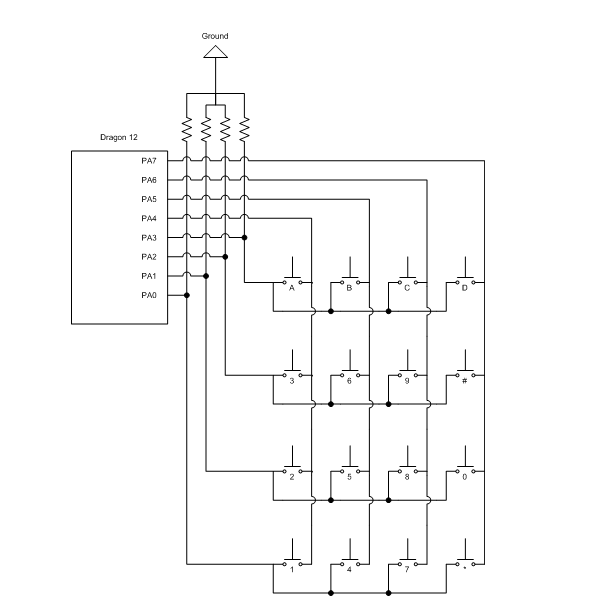
\includegraphics[scale=.85]{fig_schematic.png}\\
		
		\textbf{ \large Algorithm for reading }\\\\
		For the keypad to work, you need to set the upper four bits of DDRA as output and the lower four bits as input (0xf0). If you then set PA4 high and PA5-PA7 low, you can see that the voltage across each button in the first row (buttons 0, 1, 2, and 3) is 0V. Therefore, PA0-PA3 are all low when no keys are pressed. Pressing any of the buttons in the first row will connect the pin corresponding to that button to PA4 which is high. If you pressed any of the keys not in the first row, you would be connecting the corresponding pin to low (PA5, PA6, or PA7), and you would not be able to detect the keypress. To detect keys in another row, you need to set PA4 low and set either PA5, PA6, or PA7 high. Setting more than one of PA4, PA5, PA6 or PA7 high would make it impossible to detect exactly which key is pressed since all the keys in a column are connected to a single pin.\\
		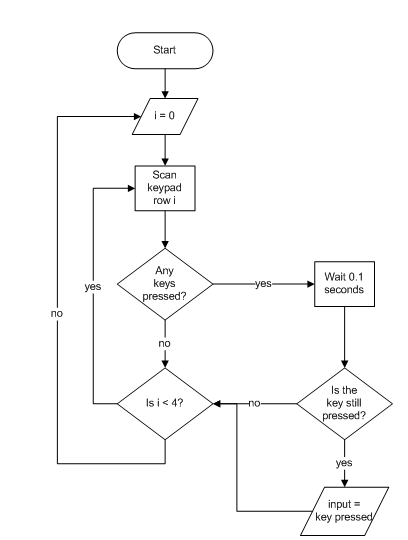
\includegraphics[scale=1]{fig_flowchart.png}\\
		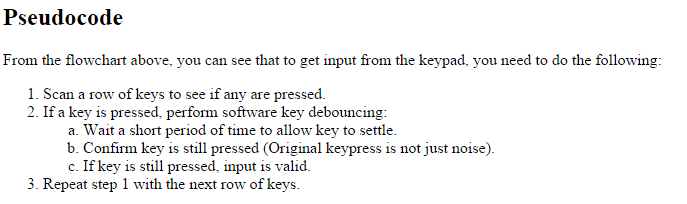
\includegraphics[scale=1]{fig_psuedocode.png}\\
\end{document}



